
\begin{figure}[t!]
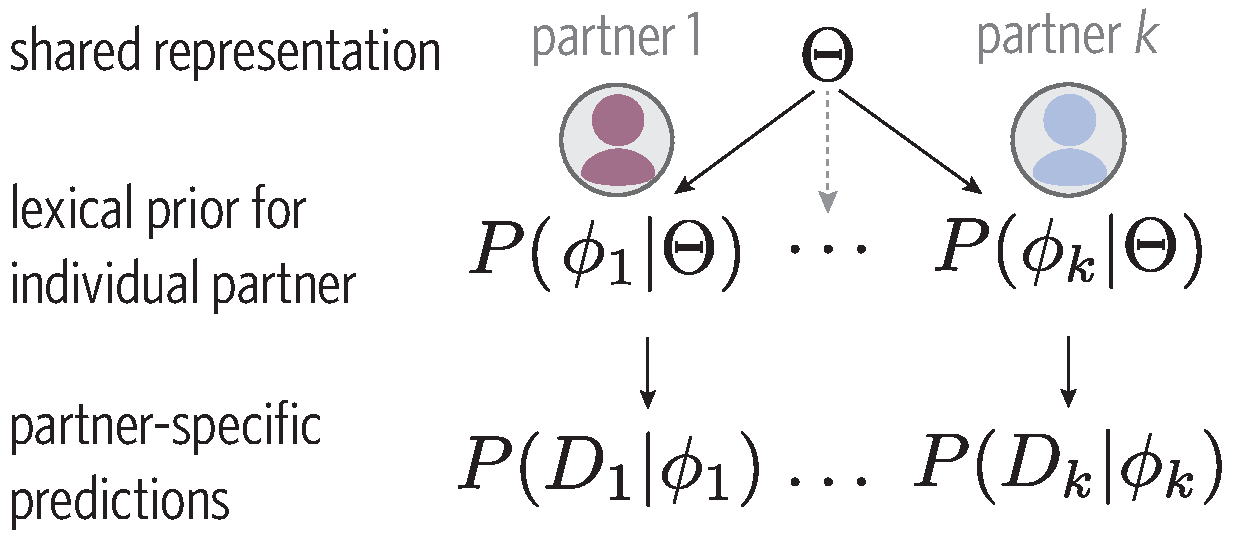
\includegraphics[scale=0.4]{./figures/task1_model.pdf}
\caption{Schematic of hierarchical Bayesian model.}
\label{fig:model_schematic}
\end{figure}

In this section, we provide an explicit computational account of the cognitive mechanisms supporting the balance between community-level stability and partner-specific flexibility.
%Our model is based on three basic principles: 
%
%\begin{enumerate}
%\item \emph{lexical uncertainty}: beliefs about the underlying conventions used by other agents are represented and updated probabilistically \cite{bergen_pragmatic_2016}
%\item \emph{pragmatic reasoning}: agents expect other agents to use language in a cooperative manner, and do so themselves  \cite{GoodmanFrank16_RSATiCS}
%\item \emph{inductive learning}: agents expect their social world to be structured, such that common beliefs may be shared even by individuals they have never met \cite{}
%\end{enumerate}
We formalize the principles of uncertainty, adaptation, and generalization in a hierarchical Bayesian model.
In a hierarchical model, the agent's uncertainty is represented by a multi-level prior. 
At the highest level of the hierarchy is \emph{community-level} uncertainty $P(\Theta)$, where $\Theta$ represents an abstract ``overhypothesis" about the overall distribution of possible partners. 
$\Theta$ then parameterizes the agent's \emph{partner-specific} uncertainty $P(\phi_{k} | \Theta)$, where $\phi_k$ represents the specific system of meaning used by partner $k$ (see Fig. \ref{fig:model_schematic}). 

Given observations $D_k$ from interactions with partner $k$, the agent updates their beliefs about the latent system of meaning using Bayes rule:
\begin{equation}
\begin{array}{rcl}
\label{eq:joint_inference}
P(\phi_k, \Theta | D_k)  & \propto &  P(D_k | \phi_k, \Theta) P(\phi_k, \Theta) \\
                           & =   & P(D_k | \phi_k) P(\phi_k | \Theta) P(\Theta)
\end{array}
\end{equation}
This joint inference decomposes the learning problem into two terms, a prior term $P(\phi_k | \Theta)P(\Theta)$ and a likelihood term $P(D_k | \phi_k)$.
The prior captures the idea that different partners may share aspects of meaning in common.
In the absence of strong evidence that partner-specific language use departs from this common structure, the agent ought to regularize toward background knowledge of the population's conventions.
The likelihood represents predictions about how a partner using a particular system of meaning will use language in context.

This joint posterior over meanings has two consequences for convention formation.
First, it allows agents to maintain partner-specific expectations $\phi_k$ by marginalizing over community-level uncertainty:
\begin{equation}
P(\phi_k | D_k) = \int_{\Theta}P(D_k | \phi_k) P(\phi_k | \Theta) P(\Theta)  d\Theta
\end{equation}
Second, the hierarchical structure provides an inductive pathway for data to inform beliefs about community-wide conventions.
Agents update their beliefs about $\Theta$ by marginalizing over data accumulated from different partners:
\begin{equation}
P(\Theta | D) = P(\Theta) \int_{\phi} P(D_k | \phi_k) P(\phi_k | \Theta) d\phi
\end{equation}
where $D = \bigcup_{k=1}^N D_k$, $\phi = \phi_1 \times \dots \times \phi_N$, and $N$ is the number of partners previous encountered. 
After multiple partners are inferred to have a similar system of meaning, beliefs about $\Theta$ shift to represent this abstracted knowledge: it becomes more likely that a novel partner will share it as well.
This transfer is sometimes referred to as ``sharing of strength'' or ``partial pooling'' because pooled data is smoothly integrated with domain-specific knowledge.

The principle of \textit{pragmatic reasoning} plays two distinct roles in our model.
First, when an agent is inferring their partner's latent representation of meaning from their observable behavior (Eq. \ref{eq:joint_inference}), we assume that the likelihood reflects Gricean principles.
In other words, the agent assumes their partner is using language in a cooperative manner.
Second, agents do not only make passive inferences from data, they actually \emph{use language} in interaction, given their current beliefs.
We assume that production and comprehension is also guided by Gricean principles.

%In this reference game setting, we can explicitly specify the likelihood and prior terms in Eq. (1). 
Concretely, we build upon the recent Rational Speech Act (RSA) framework, which formalizes the Gricean assumption of cooperativity as recursive social inference \cite{GoodmanFrank16_RSATiCS}.
A pragmatic speaker denoted by $S_1$ attempts to trade off informativity against the cost of producing an utterance, while a pragmatic listener $L_1$ inverts their generative model of the speaker to infer the intended target.
This chain of recursive reasoning grounds out in a \emph{literal listener} $L_0$, who identifies the intended target directly using a softmax over the parameterized lexical meaning function $\mathcal{L}_{\phi_k}$. 
For any utterance $u$ and world state $o$, the function $\mathcal{L}$ function returns the extent to which $u$ applies to $o$.
While this function is traditionally a binary truth-conditional variable, $\mathcal{L}_{\phi_k}: (u,o) \rightarrow \{0,1\}$, recent work has also argued for a continuous semantics mapping to the full real interval $[0,1]$  \cite{degen2020redundancy}.
This model can be formally specified as follows:
$$
\begin{array}{rcl}
L_0(o | u, \phi_k) &\propto  & \mathcal{L}_{\phi_k}(u,o) \\
S_1(u | o, \phi_k) &\propto &  \exp\{w_I \cdot \log L_0(o | u, \phi_k) - w_C \cdot c(u)\}   \\
L_1(o | u, \phi_k) &\propto  & S_1(u | o, \phi_k) P(o) 
\end{array}
$$
$c(u)$ is the cost of producing $u$ and $w_I$ and $w_C$ are free parameters controlling the relative weights on the informativity and parsimony, respectively.
Note that under each value of $\phi_k$, the $S_1$ and $L_1$ functions assign a probability to each word or object that one's partner has chosen, thus yielding the likelihood of the full set of observations $P(D_k | \phi_k)$.
In addition to using the RSA likelihood for updating an agent's beliefs about $\Theta$ and $\phi_k$, we can use the same functions to simulate the choices of speaker and listener agents on a particular trial.
That is, we sample from the posterior predictive, marginalizing over the agent's current beliefs about $\phi_k$:
\begin{align}
L(o|u) &\propto   \exp\left\{ \textstyle{\int_{\phi_k}} P(\phi_k | D_k) w_L \log S_1(u|o, \phi_k)d\phi_k\right\}\label{eq:marginalized}\\
S(u|o) &\propto  \exp\left\{ \textstyle{\int_{\phi_k}} P(\phi_k | D_k)  w_I \log L_1(o| u, \phi_k) - w_C c(u)d\phi_k\right\}\nonumber
\end{align}

\subsection{Auxiliary assumptions}

\todo[inline]{TODO: Describe more specific details that are shared across the simulations.
(1) memory discounting based on Spike, (2) lexicon prior (simplicity + space of hypotheses for each word?), (3) how we ensure normalization is well-defined w/ null utterance (i.e. handling case where a word doesn't apply to any of the objects), (4) how we handle coordination, i.e. what data is being conditioned on, (5) agent's decision rules, i.e. MAP vs. softmax sampling}

According to Spike et al., 2018 forgetting is necessary for convergence. the problem is that random guesses at the beginning of the interaction will confuse agents much later: even at the end, they'll continue to think that 4 different words can possibly refer to the same object even if only a single one has ever successfully referred to it. 

\subsection{Relation to other models}

One view this model is an argument from the continuity of probabilistic models of language acquisition in development \cite<e.g.>{XuTenenbaum07_WordLearningBayesian,FrankGoodmanTenenbaum09_Wurwur}. 
One important theoretical contribution is to generalize Bayesian models of word learning to an interactive referential setting among mature language users. 

A second view is by analogy to the use of hierarchical inference to explain how the human mind solves other difficult inductive problems in the domains of concept learning \cite{KempPerforsTenenbaum07_HBM, tenenbaum_how_2011}, causal learning \cite{KempGoodmanTenenbaum10_LearningToLearn,GoodmanUllmanTenenbaum11_TheoryOfCausality}, and speech perception \cite{kleinschmidt2015robust}.
From this view, our contribution is to ground convention formation -- a fundamentally social phenomenon -- in the same generic cognitive mechanisms supporting generalization in non-social domains, where abstract, shared properties also need to be jointly inferred with idiosyncratic particulars of instances.
The key difference is that the target of inference is the internal state of other agents; social cognition thus enters the model through the likelihood function, which represents the predictions an agent makes about how agents with different internal states are likely to behave in different contexts.


